\section{Linux Network Stack}
\textcolor{magenta}{Move to threat model}
The previous sections have demonstrated how a malicious device can take over a machine; exploiting the buggy implementation of SBP-2. In this section we introduce the notion of MMO (Motive,Means,Opportunity) in the context of DMA attacks. Using the idea we can better understand the vulnerabilities of the OS and the viability of possible prevention methods. In order to gain control over a server the malicious device needs three things:
\begin{enumerate}
    \item Motive: The device has DMA access, to what should be a restricted area. The malicious device is now motivated to exploit this situation. 
    \item Means: The device has a valid \kva of a \mabaf. The device wields the \kva as a weapon.
    \item Opportunity: The device can overwrite a callback pointer in a deterministic way. The device has a target in its cross-hairs.
\end{enumerate}
For example, a NIC has write access to a page of an RX packet. Due to sub page vulnerability a random structure with a callback pointer is accessible at a random offset. While this may seem, that the device has a valid attack vector it is actually missing two key ingredients. The device has no \textit{Means}. While the device can write a \mabaf on to the page; the device must figure out the \kva\footnote{The device is using an IOVA to access memory, to the best of our knowledge there is no way to correlate an IOVA to a \kva on a Linux machine}. The device also doesn't have an \textit{Opportunity}. Without  read access or any other additional information, the NIC cant know what structures are exposed and at what offsets. While corrupting random kernel memory may cause a kernel panic \cite{MMT16}, but its not the goal that we are after.\newline
In this section we explore new attacks on the Linux network stack; where, \textit{Means} and \textit{Opportunity} are harder to come by. 
\subsection{\shinfo}
The sk\_buff is a common data structure that is used in the Linux network stack to hold information  representing a network packet and is used by all network card drivers. Struct \skb holds the metadata of a network packet e.g., its size, associated socket and device and other important information. One of these fields, is a pointer to a data buffer. The data is usually located on a separate page (see Figure \ref{fig:sh_info}). This  separation means that \skb is never (intentionally) mapped to the device; resulting in previous works \cite{thunder} declaring that the Linux network stack is not susceptible to DMA attacks. In reality, the Linux network stack supports packet cloning by copying \footnote{\textcolor{magenta}{quote is needed}} sk\_buff metadata and letting the new one point to the same data as the old one. To support this data sharing, the \shinfo metadata structure is allocated as part of the data buffer and consequentially is always mapped to the device. Just as in the previous attack, \shinfo is unwittingly mapped for the device with the permissions of the packet i.e., write for RX packets, read for TX packets and in some cases both read and write for XDP/XSK \footnote{\url{https://www.kernel.org/doc/html/v4.18/networking/af_xdp.html}}. This design decision is the \oportunity the malicious device needs. Figure \ref{fig:sh_info} shows how a malicious device can take advantage of a \shinfo to mount an attack on the server with 4 simple steps:
\begin{enumerate}[label=(\alph*)]
    \item an RX \skb and its data buffer are allocated. The data buffer is DMA mapped for the NIC with write access (the write access is to the whole 4K page). 
    \item \textit{destructor\_arg} field in \shinfo is overwritten to point inside the mapped page. Now the \textit{destructor\_arg} is pointing to struct \uarg which is created by the NIC.
    \item \uarg has a callback pointer that is now pointing to the mallicious code that resides on the same page\footnote{In case of NX-bit, its a ROP gadget and a stack}.
    \item when \skb is freed the callback is invoked.
\end{enumerate}
This scenario assumes that the \kva of the mapped page(a.k.a \means) is known to the NIC and that \shinfo will not be overwritten by the CPU. We tackle both issues in this section.
\begin{figure}
    \centering
    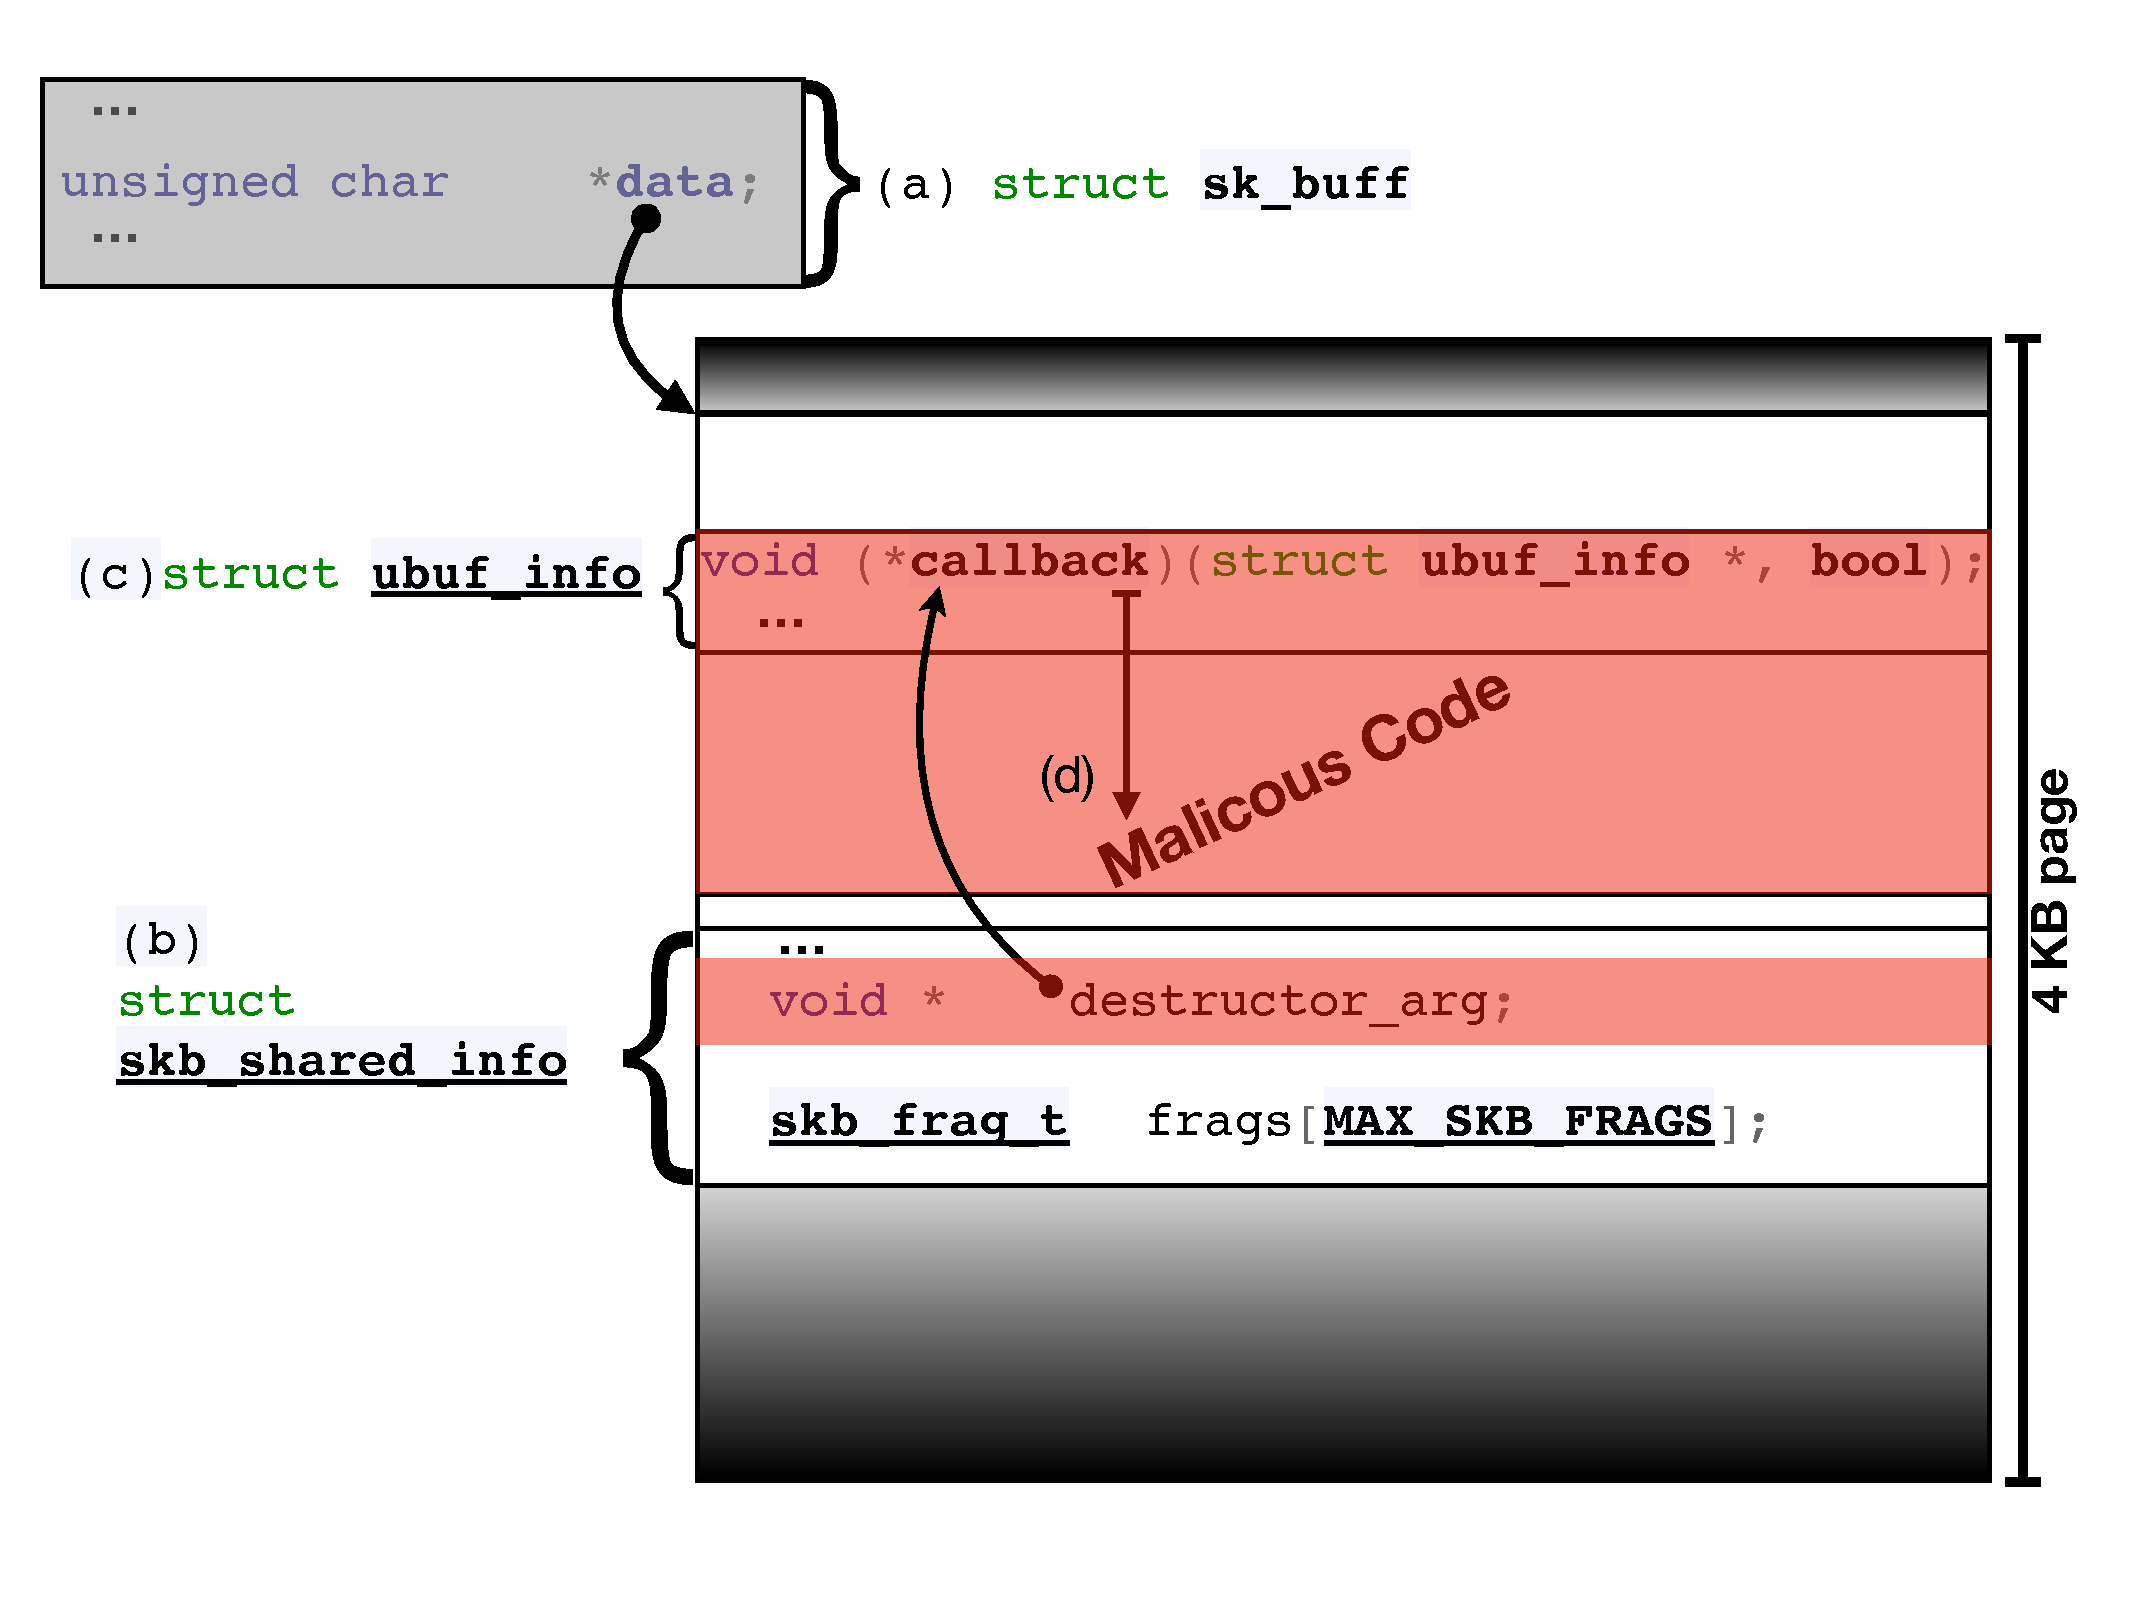
\includegraphics[width=1.1\linewidth]{figs/ubuf.pdf}
    \caption{Using \shinfo to run random code in kernel context.}
    \label{fig:sh_info}
\end{figure}

\subsection{writing \shinfo}\ref{apndx:wrong_order}
Additional challenge with attacking \shinfo is the fact the the fields are filled and rewritten by the device driver; after the packet is received. As it turns out this is not a problem as multiple device drivers \footnote{\textcolor{magenta}{make sure to get list from Gil's Thesis}} first create an skb and only then unmap, allowing the device ample opportunity to annul the changes made by the driver. But even when the order is correct; the default mode in Linux is deferred protection and though the page was unmapped the device can still access it via the IOTLB. In the case when strict protection is used; the device can rewrite \shinfo due to the way \shinfo is allocated. An RX skb is allocated via the \texttt{napi\_alloc\_skb} function\footnote{there are several other options as well, but the principle is the same} this function uses a page frag to allocate the \texttt{data} buffer that contains \shinfo. While, it is possible that the iova we were using has been invalidated, we can still access the physical page using the iova of the next RX descriptor.\textcolor{magenta}{A drawing or a description of page frag is needed, this was not clear unless youre familiar with the subject}
\begin{figure*}[t]
                \begin{lstlisting}[
        %basicstyle = \scriptsize,
        columns = flexible,
        tabsize=8,
        %frame = l,
        language = C
        ]
#define __va(x) ((void *)((unsigned long) (x)))
#define __pa(x) ((unsigned long) (x))

#define virt_to_pfn(kaddr)      (__pa(kaddr) >> PAGE_SHIFT)
#define pfn_to_virt(pfn)        __va((pfn) << PAGE_SHIFT)

        /* memmap is virtually contiguous.  */
#define __pfn_to_page(pfn)      (vmemmap + (pfn))  
#define __page_to_pfn(page)     (unsigned long)((page) - vmemmap)
                \end{lstlisting}
        \caption{ The transition between KVA, PFN and \page is just a matter of shifting bits.
                }
        \label{fig:mem_model}
\end{figure*}
\subsection{Ring Flod}
To execute a successful DMA attack on \shinfo; the attacking device needs: \begin{enumerate}
    \item a memory buffer filled with malicious code a.k.a \mabaf.
    \item the kernel virtual address of that buffer.
    \item write access to destructor\_arg field (Fig \ref{fig:sh_info})
\end{enumerate} 
Every RX packet is a possible buffer of malicious code, but the device is only given the buffer iova. The mapping between an iova and its kva is held in the device page table and the device driver meta-data; neither is accessible to the device. On RX the \texttt{struct page} address is filled by the driver(not the KVA) and additionally while we have write access we don't have read access. This means that while the \page address is in a mapped page; we cant read it because its write only. If we could read the \page address; we still wouldn't have the KVA. \newline 
Luckily for the attacker, the current memory model of x86-64 and ARM Linux servers is SPARSEMEM\_VMEMMAP \cite{mem_model}. Under this memory model the transition between KVA,PFN and \page is trivial once we have the vmem\_base value (Fig \ref{fig:mem_model}). We can guess the value of vmem\_base by looking for kernel pointers in pages mapped for TX packets.\newline 
The boot process is deterministic; executing the same set of commands, initiating the same modules and allocating the same amount of memory each reboot. While the actual pages each module gets will vary in a multi-core machine due to timing issues, the drift is not expected to be to large. We evaluate this assumptions running 128 reboots on three Dell machines with different kernel versions. In the fig\footnote{Please generate figure of RingFlod Results} we show the memory used by each driver and how many of the pfns repeat in more than X\% percent. Thus an adversary that has some knowledge about the physical setup and the kernel being used can guess with a high probability a valid kva for one of the RX pages. Whats left is to fill all the pages with a valid uarg struct with a callback pointer set back to it self, see fig \footnote{Need to generate a fig of a valid \uarg}.\textcolor{magenta}{ends to abruptly, add a sentence to tie it all back and maybe a uarg payload fig? }

\subsection{Privilege escalation}
\begin{figure*}
    \centering
    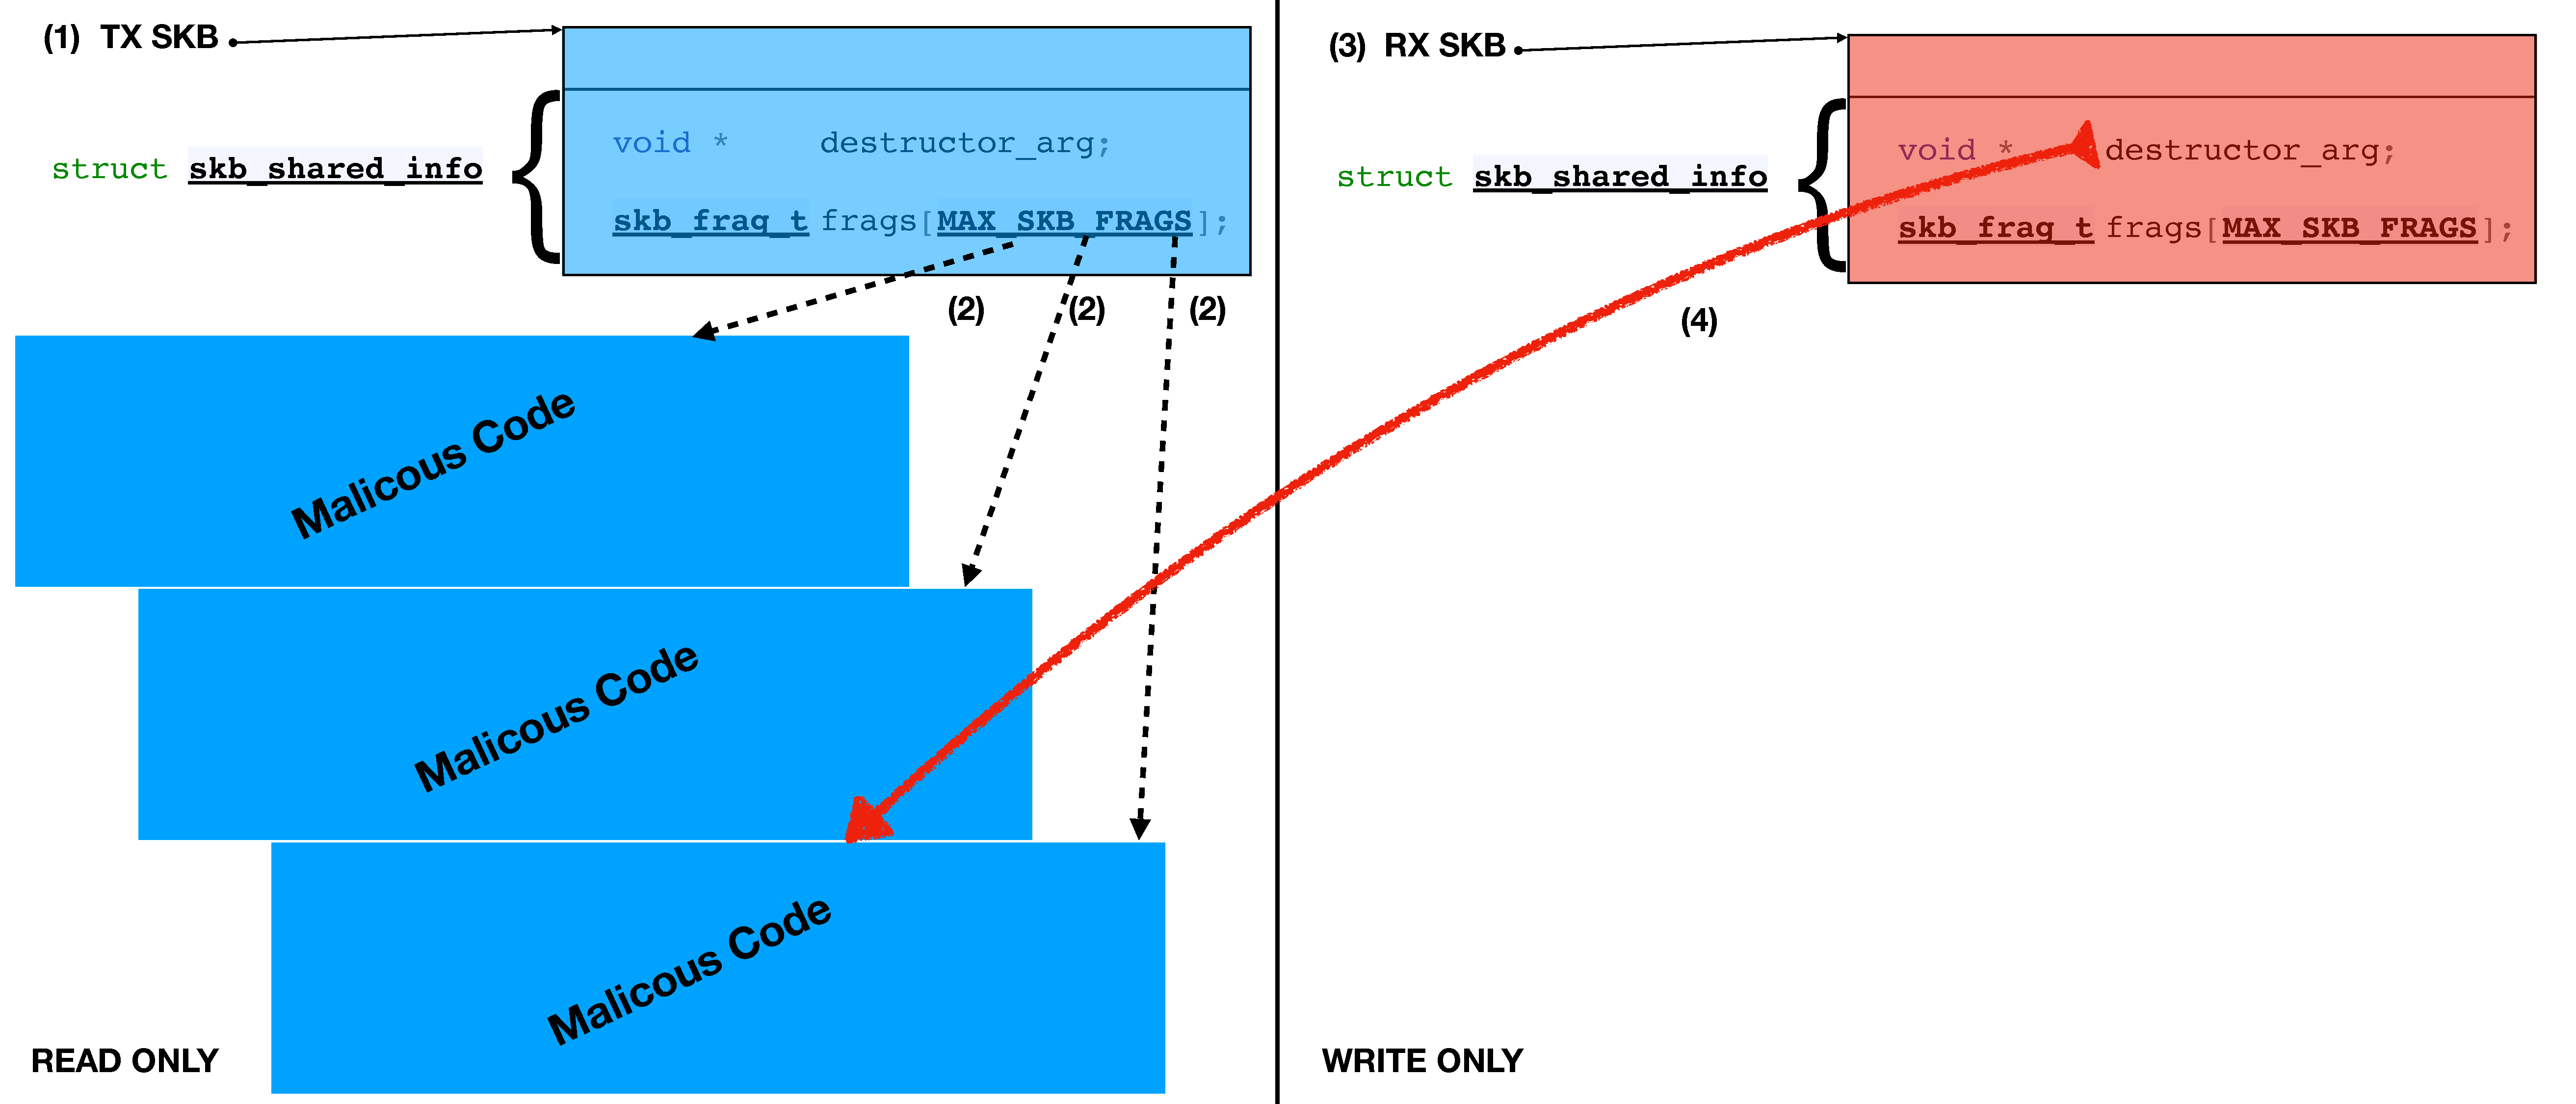
\includegraphics[width=1.1\linewidth]{figs/paylopad_both.pdf}
    \caption{An sk\_buff filled with malicious code}
    \label{fig:payload}
\end{figure*}
\shinfo of a TX packet is read only to the NIC.
But if the fragments hold malicious content; its all the malicious NIC needs for a successful attack. The readable \shinfo holds a \kva for a \page. This both allows the NIC to break KASLR and gives a \kva\footnote{\textcolor{magenta}{Do show exactly what are the KASLR bits and how you break it}} of a valid \mabaf. To implement the attack the NIC will generate an RX packet and fill the \uarg address from the calculated \kva.
The NIC will hold off on the TX completion event in order to make sure that \kva is not freed by the TX completion handler; before the poisoned RX packet is processed. A TX completion event that fails to appear in due time, will trigger a TX T/O error that will flush all buffers; the T/O is set by the driver usually to 5 seconds, which is enough to implement an attack.\newline
In this scenario the attacker doesn't need any prior knowledge of the kernel or the hardware. The only assumption is that there is an accomplice (witting or unwitting) that can open a socket in user-space. For that matter even in user-space of a guest machine; making any cloud VM a valid intrusion tool.

\subsection{Packet Forwarding}
Packet forwarding functionality is usualy disabled by default in Linux machines. But some Linux servers may function as a router or a load balancer; these machines will have packet forwarding enabled. In this scenario the NIC can independently generate an RX packets with a \mabaf. These packets can have valid 5 tuples to their network. The driver will complete the \page address of the buffer. \textcolor{red}{These packets will be forwarded and so become a TX packet that can be used as described in the previous attack.} \footnote{Need to check what happens to sh\_info, can we just forward a packet with frags (MTU, is usually a limiting factor)}

\begin{figure*}
    \centering
    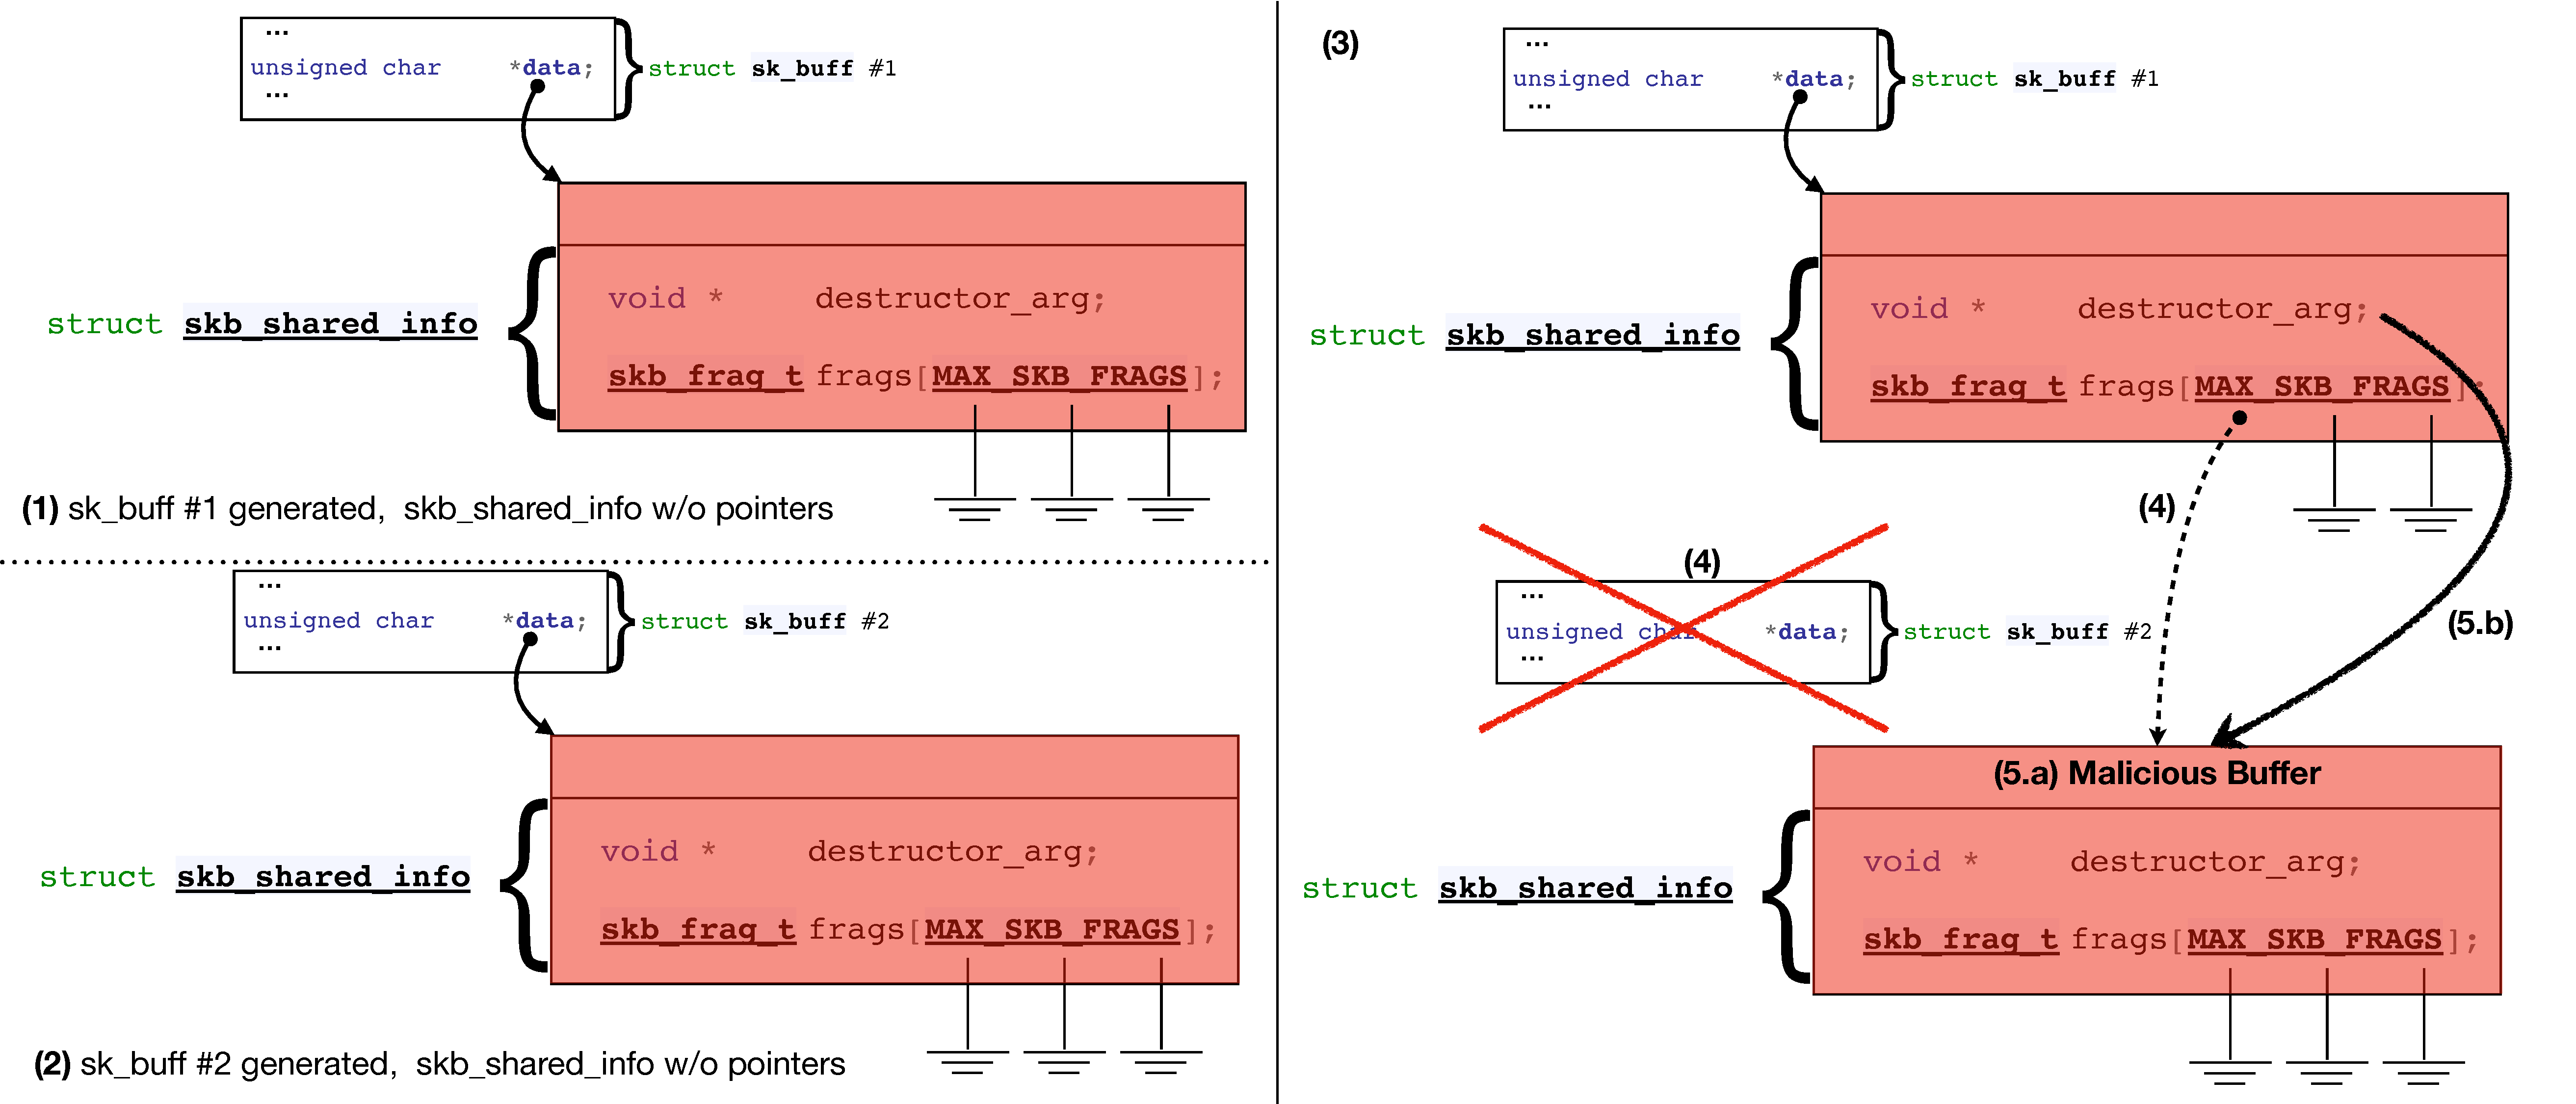
\includegraphics[width=1.1\linewidth]{figs/gro_generation.pdf}
    \caption{An sk\_buff filled with malicious code}
    \label{fig:gro}
\end{figure*}

\subsubsection{When page frags are used indiscriminately}
\textcolor{magenta}{Unfortunately the following is not found in nature... - XDP Does :)}\newline
In case where both TX and RX sh\_info come from the same page frag. The NIC can read arbitrary kernel addresses by modifying the frag list of a TX skb thus making the driver map random addresses.
Being able to read the \shinfo, allows the NIC to generate an RX packet packet with \mabaf; the \kva of which will be written by driver and read by the NIC via TX iova. From this point and on we refer the reader to the steps in the previous sections.
\subsection{XDP}
\textcolor{red}{XDP (5.1.12)is not umpapping or using DMA\_MAP\_BIDIR \- please show its ill advised...} \textcolor{magenta}{The linear skbs in mlx5 are mapping sh\_info as BI\_DIR, need to see when linear used vs non-linear and to check othe XDP drivers. When sh\_info is mapped BI\_DIR its all we need to attack.\newline
It seems linear skb (No (HW?)LRO and MTU<1500 : verify with experimnt or Boris) means no frags, while \begin{enumerate}
    \item build\_skb is used on a mapped page
    \item page is unmapped in a deferred way, regardless of iommu policy; a driver hack.
\end{enumerate} 
we cant take advantage from driver writing the \page address :( (We still can benefit from RingFlod, Escalation, Forwarding(non linear, pending experiment)). What we can do is look into \begin{enumerate}
    \item skb\_try\_coalesce
    \item SW LRO/GRO
\end{enumerate}}.
\newline
\textcolor{magenta}{In addition reviewing other drivers for the intersection of DMA\_BIDIR \^ (skb\_add\_rx\_frag||skb\_fill\_page\_descriptor)}